% DAC 2027 research manuscript (double-blind). IEEE conference format,
% 6 pages + 1 page of references.
\documentclass[conference,letterpaper]{IEEEtran}
\IEEEoverridecommandlockouts
\usepackage{cite}
\usepackage{amsmath,amssymb}
\usepackage{graphicx}
\usepackage{booktabs}
\usepackage{tabularx}
\usepackage{xcolor}
\usepackage{url}
\usepackage{balance}
\usepackage{tikz}
\usetikzlibrary{positioning,arrows.meta}
\newtheorem{proposition}{Proposition}

\begin{document}

\title{Routing, Not Reasoning: A Fail-Closed LLM Agent\\for Natural-Language Netlist Transformation}

\author{\IEEEauthorblockN{Anonymous Authors}
\IEEEauthorblockA{Paper under double-blind review}}

\maketitle

\begin{abstract}
Natural-language interfaces to EDA tools must interpret free-form requests
without compromising circuit correctness, often with models that cannot be
adapted. We present a fail-closed agent for natural-language netlist
manipulation that confines the LLM to translating each request into one intent
from a closed catalog of predefined operations. A deterministic engine executes
all circuit operations, and a mutation is committed only after a proof of
functional equivalence and checks of the operation's structural constraints;
otherwise it is rolled back. We state the assumptions under which committed
netlists remain equivalent and separate this functional guarantee from request
conformance, which it does not provide. On a 1,420-request paraphrase stress
set for the ICCAD 2026 CAD Contest Problem A, the full intent catalog reaches
88.4\% routing accuracy with gpt-4o-mini, against 61.4\% for a bare intent
list and at most 73.3\% for supervised classifiers; claude-haiku-4.5 reaches
97.4\%. Fault injection exposed one guard-bypassing operation; after its
repair, none of 24 injected faults produced an unsafe commit, while 7 produced
equivalent but non-conforming edits.
\end{abstract}

% ---------------------------------------------------------------------------
\section{Introduction}
\label{sec:intro}

Natural-language (NL) interfaces are entering EDA flows, from design question
answering to tool-script generation and RTL repair~\cite{chateda,rtlfixer,verilogeval}.
Applied to gate-level netlist manipulation, such an interface must meet two
requirements at once. First, correctness is not a quality score: a netlist
whose function has been silently altered is unusable downstream, which is why
production flows gate changes behind equivalence checking. Second, the design
state persists: requests arrive in sequence and operate on the netlist as
earlier requests left it, so an early error can shape every answer that
follows. These requirements often come with limited model capability.
Organizations that treat designs as confidential IP may prefer small, locally
deployable models~\cite{chipnemo}; benchmarks such as the ICCAD 2026 CAD
Contest Problem A~\cite{problema} mandate frozen mini-class models; and few
teams maintain a fine-tuning pipeline.

\begin{figure*}[t]
\centering
% Fig. 1 — fail-closed agent (vector, TikZ). Requires: tikz with
% positioning, arrows.meta. Units in cm; total width about 16.2 cm.
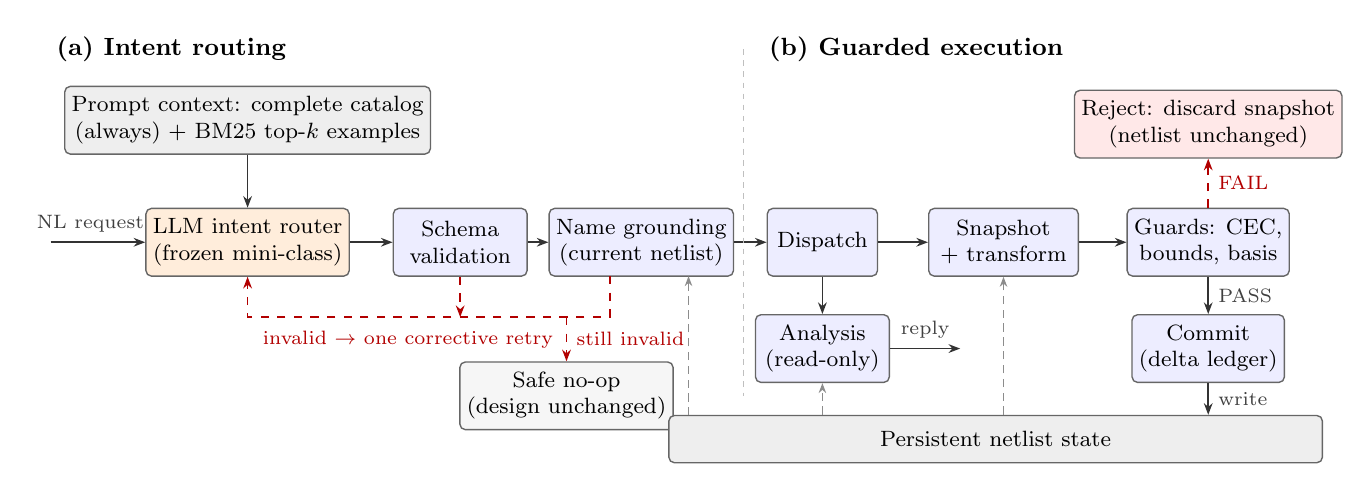
\begin{tikzpicture}[
  font=\footnotesize,
  box/.style={draw=black!60, line width=0.5pt, rounded corners=2pt,
              align=center, minimum height=0.86cm, inner sep=2.5pt},
  llm/.style={box, fill=orange!14},
  det/.style={box, fill=blue!7},
  st/.style={box, fill=gray!13},
  bad/.style={box, fill=red!9},
  flow/.style={-{Stealth[length=4.2pt]}, line width=0.6pt, black!80},
  fail/.style={-{Stealth[length=4.2pt]}, line width=0.6pt, red!70!black, dashed},
  read/.style={-{Stealth[length=3.6pt]}, line width=0.5pt, black!45, densely dashed},
  lab/.style={font=\scriptsize, text=black!75},
  flab/.style={font=\scriptsize, text=red!70!black},
]
% ---------------- main row ----------------
\node[llm, minimum width=2.3cm] (llm)    at (2.55,0)  {LLM intent router\\(frozen mini-class)};
\node[det, minimum width=1.7cm] (schema) at (5.25,0)  {Schema\\validation};
\node[det, minimum width=2.1cm] (ground) at (7.55,0)  {Name grounding\\(current netlist)};
\node[det, minimum width=1.4cm] (disp)   at (9.85,0)  {Dispatch};
\node[det, minimum width=1.9cm] (snap)   at (12.15,0) {Snapshot\\+ transform};
\node[det, minimum width=2.0cm] (guard)  at (14.75,0) {Guards: CEC,\\bounds, basis};

\draw[flow] (0.05,0) -- node[lab, above, pos=0.42] {NL request} (llm.west);
\draw[flow] (llm) -- (schema);
\draw[flow] (schema) -- (ground);
\draw[flow] (ground) -- (disp);
\draw[flow] (disp) -- (snap);
\draw[flow] (snap) -- (guard);

% ---------------- prompt context ----------------
\node[st, minimum width=3.6cm] (ctx) at (2.55,1.55)
  {Prompt context: complete catalog\\(always) + BM25 top-$k$ examples};
\draw[flow] (ctx) -- (llm);

% ---------------- single corrective-retry path ----------------
\draw[fail] (schema.south) -- (5.25,-0.95);
\draw[fail] (7.15,-0.43) -- (7.15,-0.95) -- (2.55,-0.95) -- (llm.south);
\node[flab, anchor=north west] at (2.62,-1.0) {invalid $\rightarrow$ one corrective retry};
\node[box, fill=gray!7, minimum width=2.2cm] (noop) at (6.6,-1.95)
  {Safe no-op\\(design unchanged)};
\draw[fail] (6.6,-0.95) -- node[flab, right] {still invalid} (noop.north);

% ---------------- analysis branch ----------------
\node[det, minimum width=1.7cm] (ana) at (9.85,-1.35) {Analysis\\(read-only)};
\draw[flow] (disp) -- (ana);
\draw[flow] (ana.east) -- node[lab, above] {reply} (11.6,-1.35);

% ---------------- guarded commit ----------------
\node[det, minimum width=1.7cm] (commit) at (14.75,-1.35) {Commit\\(delta ledger)};
\draw[flow] (guard) -- node[lab, right] {PASS} (commit);
\node[bad, minimum width=2.4cm] (rej) at (14.75,1.5)
  {Reject: discard snapshot\\(netlist unchanged)};
\draw[fail] (guard) -- node[flab, right] {FAIL} (rej);

% ---------------- persistent state ----------------
\node[st, minimum width=8.3cm, minimum height=0.6cm] (state) at (12.05,-2.5)
  {Persistent netlist state};
\draw[read] (8.15,-2.2) -- (8.15,-0.43);
\draw[read] (state.north -| ana) -- (ana.south);
\draw[read] (state.north -| snap) -- (snap.south);
\draw[flow] (commit) -- node[lab, right] {write} (state.north -| commit);

% ---------------- region titles ----------------
\draw[black!25, dash pattern=on 2pt off 2pt] (8.85,2.45) -- (8.85,-1.95);
\node[font=\small\bfseries, anchor=west] at (0.0,2.45) {(a) Intent routing};
\node[font=\small\bfseries, anchor=west] at (9.05,2.45) {(b) Guarded execution};
\end{tikzpicture}

\caption{Overview of the fail-closed netlist agent. (a)~The LLM maps each
natural-language request to an intent, using the complete operation catalog
and additional BM25-retrieved demonstrations. Schema validation and grounding
against the current netlist allow one corrective retry; a request that is
still invalid yields a safe no-op. (b)~Read-only queries execute directly,
whereas mutations operate on a snapshot and commit only after the equivalence
and structural checks pass; rejected candidates leave the persistent netlist
unchanged. Dashed gray arrows: reads of the current netlist.}
\label{fig:arch}
\end{figure*}

When the LLM itself generates the executable artifact---a tool script, an
edited netlist, or RTL code---its errors have a direct path into the design.
Post-hoc checks catch many of them, but the failure surface is hard to bound,
and a smaller model raises the error rate the checks must absorb.

We take the opposite approach: the LLM routes; it does not rewrite. Its only
output is one intent object per request, drawn from a closed catalog of about
80 predefined operations with typed parameters. A deterministic engine
performs every circuit operation. Parameters that name nets or gates are
grounded against the current netlist before execution, and each mutation runs
on a snapshot that is committed only after a proof of functional equivalence,
obtained through a register-cut projection, and checks of the operation's
structural constraints; otherwise the snapshot is restored.

This architecture bounds what the LLM can damage, but not what it can
misunderstand. Under explicitly stated assumptions, every committed netlist is
functionally equivalent to its predecessor; a mis-routed request can still
commit a valid but unwanted edit, and that edit persists into later requests.
We therefore evaluate both sides: how accurately small frozen models route
requests, and which faults the guards prevent and which they cannot.

Our contributions are:
\begin{itemize}
\item \textbf{Architecture.} A constrained interface for NL netlist
  manipulation that separates LLM intent interpretation from deterministic
  execution and proof-gated commit, with an explicit statement of what it
  guarantees (functional integrity, under stated assumptions) and what it does
  not (request conformance) (Section~\ref{sec:design}).
\item \textbf{Routing evaluation.} A controlled study on 1,420 paraphrased
  requests that compares a bare intent list, a full catalog, retrieval
  configurations, model choices, and supervised baselines, and analyzes the
  near-synonym operations behind most residual errors
  (Sections~\ref{sec:routing-acc}--\ref{sec:failures}).
\item \textbf{Validation and limits.} Fault injection and the official contest
  evaluation, quantifying prevented violations, residual semantic drift, and
  one guard-bypassing operation that the experiment exposed and that we
  repaired (Sections~\ref{sec:fault}--\ref{sec:official}).
\end{itemize}

% ---------------------------------------------------------------------------
\section{Problem Setting and Related Work}
\label{sec:related}

\textbf{Setting.} A session loads one flat gate-level Verilog netlist---two-input
primitive gates, inverters, buffers, and D flip-flops with asynchronous
control---and then receives free-form NL requests, one per line, answered in
lock-step~\cite{problema}. Requests analyze (depth, cones, paths, equivalence),
edit (buffer insertion, basis conversion, renaming), or optimize (depth, gate
count) the current netlist. Hard requirements---functional equivalence where
requested, stated structural bounds, gate-basis restrictions---are
all-or-nothing: violating any one zeroes the testcase.

\textbf{LLM agents for EDA.} Script-generating agents emit tool scripts for EDA
flows and check them before execution~\cite{chateda,jarvis,openroadagent};
flow-tuning agents search a bounded parameter space~\cite{orfsagent,statetune};
FluxEDA keeps backend instances alive so that later steps observe earlier
state~\cite{fluxeda}. RTL-oriented work generates or repairs code against
compilers and testbenches~\cite{rtlfixer,verilogeval,rtllm}, and recent
benchmarks target netlist manipulation and tool
calling~\cite{netlistbench,mcpbench}. These systems differ in how much
execution freedom the LLM holds; in ours it holds none beyond selecting one
predefined operation and its parameters on a persistent gate-level netlist.

\textbf{Structured tool calling.} Schema-constrained function calling is well
established~\cite{gorilla,toolllm,bfcl}, typically retrieving tool
documentation into the prompt. We instead retrieve labeled example requests,
keep the full catalog in every prompt, and validate name-typed parameters
against a design state that earlier requests have modified.

\textbf{Verified and checked execution.} LLM-Modulo argues for LLM generation
behind external verifiers~\cite{llmmodulo}; obligation and transaction checks
constrain agent actions outside EDA~\cite{refineact,toolgate,taubench}.
Concurrent work on the same benchmark shows that a run passing every
equivalence check can still contain incorrect answers and violated
constraints, and adds request-derived completion checks~\cite{companion}. That
work checks conformance, whereas ours bounds functional damage; the two are
complementary. Our contribution is therefore not a new verification primitive
but a commit protocol for persistent sequential netlists, state-aware
parameter grounding, and a measured account of what the combination prevents.

% ---------------------------------------------------------------------------
\section{Fail-Closed Agent Design}
\label{sec:design}


\subsection{Closed-World Intent Interface}
\label{sec:interface}

The catalog defines about 80 intents covering analysis (counts, depth, cones,
paths, connectivity, functional properties), transformation (basis remapping,
buffer insertion, cleanup, renaming), and optimization (depth, gate count).
Each intent declares required and optional parameters with types; enumerated
parameters such as the gate basis have closed value sets. The catalog
text---a description of each intent plus disambiguation entries for
operations that users phrase similarly---is part of every prompt as a fixed,
cacheable prefix of about 12.8k tokens. Retrieval only adds examples and never
removes catalog entries, so a retrieval miss cannot put the correct operation
out of the model's reach.

The operation space is closed; the parameter space is not. Which net, cone,
bound, or basis an operation applies to is decided per request. A request that
maps to no catalog operation yields a safe no-op that reports the design
unchanged. Extending the catalog means adding a handler, a schema, and a
disambiguation entry---an auditable engineering change rather than model
retraining.

\subsection{Routing with Live-State Grounding}
\label{sec:routing}

Routing proceeds in four stages (Fig.~\ref{fig:arch}a).
(1)~\emph{Translation:} the LLM receives the catalog and the 50 most similar
labeled requests, retrieved by BM25 from a bank of 940 requests drawn from the
contest's public and beta rounds, and emits one JSON intent object.
(2)~\emph{Schema validation:} an unknown intent, a missing parameter, or an
illegal enumerated value is rejected, and the rejection reason is returned to
the LLM for one corrective retry. (3)~\emph{Name grounding:} every parameter
that must name a net, gate, or flip-flop is checked against the current
netlist, which earlier requests may have modified; a nonexistent name triggers
re-translation with the error message. (4)~\emph{Dispatch} to a deterministic
handler: analysis handlers run graph algorithms on the netlist IR, and
mutation handlers enter the commit protocol of Section~\ref{sec:commit}.
Translations are cached within a session, and if every stage fails the agent
returns the safe no-op.

\subsection{Guarded Execution and Commit Protocol}
\label{sec:commit}

A mutation handler transforms a snapshot of the netlist
(Fig.~\ref{fig:arch}b), and three checks decide whether the snapshot replaces
the current design.
\begin{enumerate}
\item \textbf{Functional equivalence.} A register-cut projection turns the
  sequential netlist into a combinational one: each flip-flop's D, CK, RN, and
  SN pins become pseudo-outputs and its Q pin a pseudo-input. Flip-flops
  correspond by instance identity, and a change to the register set is
  rejected outright. Because every flip-flop input is observed, combinational
  equivalence of the projections implies sequential equivalence for the
  testbed's flip-flop model, including logic on clock and asynchronous pins.
  ABC's \texttt{cec} decides equivalence~\cite{abc}, with a yosys check as a
  fallback.
\item \textbf{Structural bounds.} Bounds carried by the operation, such as a
  maximum fanout, are recomputed on the result.
\item \textbf{Basis purity.} If the operation restricts gate types, the
  gate-type set of the result is checked.
\end{enumerate}
The acceptance rule is fail-closed: the snapshot is committed only when every
check passes and equivalence is proved. A disproof, a timeout, or an
inconclusive result---for instance on a malformed netlist---restores the
snapshot. Candidates produced by the optimizer, including precomputed
candidates that serve as search seeds, obey the same rule. Committed mutations
are recorded in a delta ledger that later requests (``how many buffers were
added?'') query.

\subsection{Scope of the Guarantee}
\label{sec:scope}

We distinguish three properties of a committed edit: \emph{functional
integrity} (the netlist computes the same function), \emph{structural
validity} (it meets the bounds and basis of the routed operation), and
\emph{request conformance} (the routed operation is what the user asked for).
Every mutation intent in the catalog is function-preserving by specification;
a request that would change function (e.g., inserting a gating cell) has no
catalog operation and cannot be executed as requested. The architecture targets
the first two properties, under four assumptions:
\begin{itemize}
\item \textbf{(A1) Complete mediation.} Every operation that mutates the
  netlist, including renaming, executes through the commit protocol.
\item \textbf{(A2) Sound checking.} A proof of equivalence reported by the
  checker is correct for the projected circuits.
\item \textbf{(A3) Faithful projection.} The register-cut model matches the
  flip-flop semantics of the netlist.
\item \textbf{(A4) Correct structural checks.} The bound and basis checks accept
  a netlist only if it meets the bounds and basis carried by the operation.
\end{itemize}

\begin{proposition}
Under A1--A4, every netlist the agent commits is functionally equivalent to the
netlist it replaces, and hence to the most recently loaded design, and meets
the bounds and basis of the routed operation. An inconclusive check never
produces a commit.
\end{proposition}
\begin{IEEEproof}[Proof sketch]
By A1, the current netlist changes only when a snapshot is committed, and a
commit requires a proof of equivalence of the register-cut projections and
passing structural checks. By A2 the proof is correct for the projections, by
A3 projection equivalence implies sequential equivalence, and by A4 the
structural checks are correct. Equivalence is transitive, so induction over the
sequence of commits extends it to the loaded design. A disproof, a timeout, or
an inconclusive result restores the snapshot by the acceptance rule.
\end{IEEEproof}
The proposition says nothing about request conformance: a mis-routed request can commit an equivalent
but unwanted edit, and because the design persists, that edit changes what
later requests observe---for example, a gate count or a net name that a later
question depends on. The guards also enforce only the requirements carried by
the current operation, not constraints established by earlier requests. A1 is
the assumption most exposed to implementation error, and
Section~\ref{sec:fault} tests it directly.

% ---------------------------------------------------------------------------
\section{Evaluation}
\label{sec:eval}

\subsection{Setup}
\label{sec:setup}

\textbf{Requests.} We evaluate routing on a stress set of 1,420 requests that
our team wrote during the contest by paraphrasing the official request
patterns: 71 operations with 20 paraphrases each, of which 1,065 use
deliberately indirect or unusual wording and 355 use standard phrasing. The
set provides ground-truth intents and parameters but no netlists, so we score
the translation output directly. The retrieval bank of 940 requests from the
contest's public and beta rounds is disjoint from the stress set. A second,
high-recall bank of 2,130 author-written paraphrases contains paraphrases of
the same operations as each test request; we use it with
leave-one-testcase-out (LOCO) exclusion and only as an upper bound, because it
shares the stress set's distribution. Since the catalog's disambiguation
entries were refined during the contest while inspecting errors on this set,
accuracies on it may be optimistic.

\textbf{Metric and models.} The primary metric is intent accuracy: whether the
selected operation is correct. We use the two contest-mandated models,
gpt-4o-mini and claude-haiku-4.5, at temperature 0.2, and repeat the
gpt-4o-mini headline settings five times ($N{=}5$). Evaluation rounds run
strictly one at a time, and any round with a degraded API call is discarded,
because rate limiting can silently turn LLM calls into no-op responses.

\subsection{Routing Accuracy}
\label{sec:routing-acc}

\begin{table}[t]
\caption{Intent routing accuracy on the 1,420-request stress set (means over
$N$ runs). Exact obj.: intent and all parameters correct. Bank: source of the
BM25-retrieved examples ($k{=}50$).}
\label{tab:routing}
\centering
\footnotesize
\setlength{\tabcolsep}{3pt}
\begin{tabularx}{\columnwidth}{@{}l>{\raggedright\arraybackslash}Xrrc@{}}
\toprule
Method & Configuration & Intent & Exact obj. & $N$ \\
\midrule
\multicolumn{5}{@{}l}{\emph{Non-LLM baselines}} \\
BM25 NN & production bank & 47.4\% & -- & -- \\
SBERT + kNN & all labels, LOCO & 72.8\% & -- & -- \\
TF-IDF + SVM & all labels, LOCO & 73.3\% & -- & -- \\
\midrule
\multicolumn{5}{@{}l}{\emph{LLM-based routing}} \\
gpt-4o-mini & bare intent list & 61.4\% & 55.4\% & 3 \\
claude-haiku-4.5 & bare intent list & 78.7\% & 72.3\% & 1 \\
gpt-4o-mini & full catalog & 88.4\% & 79.5\% & 5 \\
claude-haiku-4.5 & full catalog & 96.4\% & 91.4\% & 3 \\
gpt-4o-mini & catalog + production bank & 88.9\% & 82.0\% & 5 \\
gpt-4o-mini & catalog + high-recall bank$^\dagger$ & 95.4\% & 91.6\% & 2 \\
claude-haiku-4.5 & catalog + production bank & 97.4\% & 92.7\% & 1 \\
\bottomrule
\end{tabularx}

\vspace{2pt}
\parbox{\columnwidth}{\footnotesize Min--max over runs: gpt-4o-mini bare 61.1--61.8,
full catalog 88.3--88.7, production bank 88.6--89.2, high-recall bank
95.1--95.6; claude-haiku-4.5 full catalog 96.3--96.5. $^\dagger$Upper bound: the bank
shares the stress set's distribution. LOCO: leave-one-testcase-out.}
\end{table}

\textbf{Catalog information is the largest lever.} A bare list of intent names
yields 61.4\% with gpt-4o-mini; the full catalog---descriptions, parameter
schemas, and disambiguation entries together---raises it to 88.4\% (+27.0
points). The bare condition keeps the schema-feedback retry, whose fixed
message mentions class-level depth intents, and contains no other catalog
text. The gap between the two models is 17.3 points with the bare list but 8.0
points with the full catalog, so the catalog helps the weaker model more.

\textbf{Supervised baselines underperform.} With every labeled request
available, the best classifier reaches 73.3\% (TF-IDF features with a linear
SVM), and frozen sentence embeddings reach 72.8\%. Classifiers and LLMs are
scored on the same operation-level metric; the LLM additionally fills in
parameters (84.6\% parameter accuracy for gpt-4o-mini with the catalog,
94.1\% for claude-haiku-4.5 with retrieval), which the classifiers do not
attempt. With only the production bank, three operations have no examples and
are unreachable for nearest-neighbor routing, whereas the LLM reaches them
through the catalog.

\textbf{Retrieval adds little with the production bank.} Retrieving $k{=}50$
examples from the production bank adds 0.5 points for gpt-4o-mini and 1.0
point for claude-haiku-4.5 over the catalog alone, and retrieval depth barely
matters: for gpt-4o-mini, $k$ from 5 to 100 spans 88.1--89.4\% without a
monotone trend, while label recall rises from 60\% to 86\%. The catalog thus
carries most of the routing accuracy: claude-haiku-4.5 reaches 96.4\% with no
retrieval at all, even though the production bank's label recall at $k{=}50$
is only 82.1\%. Retrieval pays off only when the examples closely match the
requests: the high-recall bank adds 6.4 points for gpt-4o-mini, an upper bound
because it shares the stress set's distribution, and an effect comparable to
switching models (+8.0 points with the catalog alone).

\subsection{Failure Analysis}
\label{sec:failures}

Moving gpt-4o-mini from the production to the high-recall bank removes 84\% of
give-ups (44 to 7) but only 43\% of wrong-operation picks (110 to 63): good
examples mainly help the model recognize unfamiliar phrasing. What remains is
dominated by confusions between semantically similar operations, such as
primary-input-to-output depth versus global maximum depth, or floating versus
dangling nets, and part of it reflects genuine ambiguity in the requests. The
supervised baselines confuse the same operation families. The concurrent
agent of~\cite{companion}, built on a different architecture, reports the same
kind of scope error on this benchmark (a pairwise depth of 10 reported as the
whole-design depth of 53). On this request distribution, near-synonym
discrimination is a major source of residual routing errors.

\subsection{Fault Injection}
\label{sec:fault}

\begin{table}[t]
\caption{Fault-injection outcomes. Routing faults corrupt the router's output
at dispatch; engine faults corrupt a transformation inside the engine. Classes
are mutually exclusive.}
\label{tab:fault}
\centering
\footnotesize
\setlength{\tabcolsep}{3pt}
\begin{tabularx}{\columnwidth}{@{}l>{\raggedright\arraybackslash}Xccc@{}}
\toprule
 & & \multicolumn{2}{c}{Routing (21)} & Engine (3) \\
\cmidrule(lr){3-4}\cmidrule(l){5-5}
Outcome & Meaning & before fix & after fix & \\
\midrule
Rejected & refused before execution & 2 & 5 & 0 \\
Rolled back & equivalence disproved & 0 & 0 & 3 \\
Benign & met every hard requirement & 9 & 9 & 0 \\
Drift & equivalent but non-conforming & 7 & 7 & 0 \\
Unsafe & non-equivalent netlist committed & 3 & 0 & 0 \\
\bottomrule
\end{tabularx}
\end{table}

To test A1 and the guards, we use two fault models. \emph{Routing faults}
corrupt the router's output at the dispatch layer, simulating worst-case LLM
behavior: numeric bounds off by one in either direction, a wrong but
implemented basis or transformation, a basis outside the closed world, a
target redirected to a different existing net, and a swap to a different
intent. \emph{Engine faults} instead inject a function-changing rewire inside
a transformation, standing in for an implementation bug. We run 24 injections
(21 routing, 3 engine) over six transformation-heavy public testcases (the six
uncorrupted runs pass all checks) and classify each final netlist against the
hard requirements of the original request (Table~\ref{tab:fault}).

The two fault models are stopped by different mechanisms. Every rollback came
from an engine fault: the equivalence check caught all three function-changing
rewires. No routing fault produced a function-changing edit through the commit
protocol, because every catalog operation preserves function; routing faults
were either refused by the closed world or yielded an equivalent netlist. Only
rejections and rollbacks are detections; the nine benign cases passed
because the corrupted edit happened to remain acceptable. The three unsafe
commits shared one cause, a violation of A1: renaming was treated as cosmetic
and bypassed the commit protocol, so renaming a net onto an existing name
merged two drivers while the agent reported success. In one of these cases ABC
returned an inconclusive result on the double-driven net, which an evaluation
harness that treats inconclusive results as passing would have accepted.
After we added a check that rejects renames onto existing names, no injection
produced an unsafe commit, and the 40 public testcases pass all 84 of their
hard-requirement checks. The seven drift cases mark the conformance boundary
of Section~\ref{sec:scope}: the guards enforced the corrupted operation's
contract rather than the user's sentence, and the response claimed success.
Detecting them requires request-level completion checks such as those
of~\cite{companion}. Because the design persists, a single corrupted request
also changes later answers: in 13 of the 24 runs, at least one later response
differs from the uncorrupted run (27 of 173 later responses). This happens even
when the guards act, since a refused or rolled-back request leaves the design
in a state the user did not intend; the later answers are then correct for the
actual design, whereas after drift the agent had reported success.

\subsection{Official Evaluation and Post-Contest Analysis}
\label{sec:official}

In the contest's final round (100 testcases and 674 requests, unseen during
development), the submitted configuration met every hard requirement and
scored 671.366 of 674 under official scoring. All losses came from
optimization requests, which are scored by their cost relative to the best
cost among all entries. Table~\ref{tab:official} compares the official result
with two post-contest re-evaluations of the same 46 optimization requests.

\begin{table}[t]
\caption{Optimization performance on the 46 final-round optimization requests.
Normalized score: mean request score $\times$ 100\%.}
\label{tab:official}
\centering
\footnotesize
\setlength{\tabcolsep}{3pt}
\begin{tabularx}{\columnwidth}{@{}lc>{\raggedright\arraybackslash}X@{}}
\toprule
Configuration & Normalized score & Compute \\
\midrule
Official evaluation & 94.27\% & $1\times$ (300\,s per request) \\
Re-run, same configuration & 94.60\% & $1\times$ \\
Best of up to four runs$^\dagger$ & 95.62\% & up to $4\times$ \\
\bottomrule
\end{tabularx}

\vspace{2pt}
\parbox{\columnwidth}{\footnotesize $^\dagger$Post-contest upper bound;
includes an earlier engine version.}
\end{table}

A single re-run under the same per-request budget improves 15 requests and
worsens 4, for a net gain of 0.32 percentage points: the optimizer's search is budget-bound and
stochastic, and one run is far from its best achievable result. Taking the
best of up to four runs, at up to four times the compute, adds 1.34
percentage points; all 17
improved netlists were re-verified independently with ABC, and four of them
beat the best cost among all contest entries. These figures are post-contest
upper bounds, not a comparison under the official protocol. Three requests
resist re-sampling entirely (3.1 percentage points) and call for algorithmic
improvement.

% ---------------------------------------------------------------------------
% \balance must sit in the left column of the last text page; move it if the layout changes.
\balance
\section{Limitations and Conclusion}
\label{sec:conclusion}

\textbf{Limitations.} We evaluate on one benchmark. The routing stress set was
written by the authors and the catalog refined against it, so its accuracies
may be optimistic; the official final round provides an out-of-sample,
end-to-end check. The cloud mini-class models stand in for the small, locally
deployable models that motivate this work, and direct validation on
open-weight models remains future work. Some settings were run once
($N{=}1$). The functional guarantee rests on A1--A4 and on a correct
implementation of them, and drift---valid but non-conforming edits---is
outside its scope.

\textbf{Conclusion.} Restricting the LLM to selecting predefined operations,
and committing their results only on proof, bounds the functional damage that
an LLM error can cause in persistent netlist manipulation, under assumptions
that can be stated and tested; fault injection found and closed a gap in the
assumption most exposed to implementation error. What the architecture does
not bound---whether the executed operation is the one the user meant---remains,
and our routing study locates most of it in near-synonym operations. For
agents that edit an existing design, safe execution and request conformance
are separate problems, and each needs explicit treatment.

\section*{Acknowledgment}
AI coding assistants were used for implementation, data post-processing, and
language editing; all AI-assisted output was reviewed and revised by the
authors, who take full responsibility for the content.

% ---------------------------------------------------------------------------
\clearpage
\begin{thebibliography}{99}
\bibitem{chateda} H.~Wu, Z.~He, X.~Zhang, X.~Yao, S.~Zheng, H.~Zheng, and B.~Yu, ``ChatEDA: A large language model powered autonomous agent for EDA,'' \emph{IEEE Trans. Comput.-Aided Design Integr. Circuits Syst.}, vol.~43, no.~10, pp.~3184--3197, 2024.
\bibitem{rtlfixer} Y.~Tsai, M.~Liu, and H.~Ren, ``RTLFixer: Automatically fixing RTL syntax errors with large language models,'' in \emph{Proc. DAC}, 2024.
\bibitem{verilogeval} M.~Liu, N.~Pinckney, B.~Khailany, and H.~Ren, ``VerilogEval: Evaluating large language models for Verilog code generation,'' in \emph{Proc. ICCAD}, 2023.
\bibitem{chipnemo} M.~Liu \emph{et al.}, ``ChipNeMo: Domain-adapted LLMs for chip design,'' arXiv:2311.00176, 2023.
\bibitem{problema} C.-H.~Chou, H.-C.~Chiu, C.-J.~Hsu, and Y.~Liu, ``ICCAD Contest Problem A: LLM-assisted netlist exploration and transformation,'' problem specification and Q\&A, 2026.
\bibitem{jarvis} G.~Pasandi \emph{et al.}, ``JARVIS: A multi-agent code assistant for high-quality EDA script generation,'' arXiv:2505.14978, 2025.
\bibitem{openroadagent} B.-Y.~Wu, U.~Sharma, A.~Rovinski, and V.~A.~Chhabria, ``OpenROAD Agent: An intelligent self-correcting script generator for OpenROAD,'' in \emph{Proc. IEEE ICLAD}, 2025, pp.~16--22.
\bibitem{orfsagent} A.~Ghose, A.~B.~Kahng, S.~Kundu, and Z.~Wang, ``ORFS-agent: Tool-using agents for chip design optimization,'' in \emph{Proc. ACM/IEEE MLCAD}, 2025, pp.~1--13.
\bibitem{statetune} K.~Li, S.~Yao, S.~Zheng, and L.~Wang, ``StateTune: Transforming LLM-assisted EDA flow tuning into a stateful, closed-loop process,'' in \emph{Proc. IEEE/ACM ICCAD}, 2026.
\bibitem{fluxeda} Z.~Chen, Z.~Song, Y.~Li, Q.~Sun, and C.~Zhuo, ``FluxEDA: A unified execution infrastructure for stateful agentic EDA,'' arXiv:2603.25243, 2026.
\bibitem{rtllm} Y.~Lu, S.~Liu, Q.~Zhang, and Z.~Xie, ``RTLLM: An open-source benchmark for design RTL generation with large language model,'' in \emph{Proc. ASP-DAC}, 2024.
\bibitem{netlistbench} J.~Ma, J.~Wang, Y.~Ma, Z.~Zhuang, and X.~Liu, ``NetlistBench: Evaluating LLM reliability in SPICE netlist recognition and manipulation,'' arXiv:2608.12197, 2026.
\bibitem{mcpbench} F.~Liparulo and F.~Pierri, ``Benchmarking AI agents for hardware design automation via MCP tool calling,'' arXiv:2608.26199, 2026.
\bibitem{gorilla} S.~G.~Patil, T.~Zhang, X.~Wang, and J.~E.~Gonzalez, ``Gorilla: Large language model connected with massive APIs,'' in \emph{Proc. NeurIPS}, 2024.
\bibitem{toolllm} Y.~Qin \emph{et al.}, ``ToolLLM: Facilitating large language models to master 16000+ real-world APIs,'' in \emph{Proc. ICLR}, 2024.
\bibitem{bfcl} S.~G.~Patil \emph{et al.}, ``The Berkeley Function Calling Leaderboard (BFCL): From tool use to agentic evaluation of large language models,'' in \emph{Proc. ICML}, 2025.
\bibitem{llmmodulo} S.~Kambhampati \emph{et al.}, ``Position: LLMs can't plan, but can help planning in LLM-Modulo frameworks,'' in \emph{Proc. ICML}, 2024.
\bibitem{refineact} F.~Batole, F.~Khomh, and H.~Rajan, ``RefineAct: Automatic runtime verification of LLM agent actions,'' in \emph{Proc. IEEE/ACM ASE}, 2026.
\bibitem{toolgate} Y.~Liu \emph{et al.}, ``ToolGate: Contract-grounded and verified tool execution for LLMs,'' in \emph{Findings of ACL}, 2026, pp.~9653--9684.
\bibitem{taubench} S.~Yao, N.~Shinn, P.~Razavi, and K.~Narasimhan, ``$\tau$-bench: A benchmark for tool-agent-user interaction in real-world domains,'' in \emph{Proc. ICLR}, 2025.
\bibitem{companion} ``Beyond equivalence: Checking task completion in LLM-based netlist analysis, editing, and optimization,'' concurrent submission, 2026.
\bibitem{abc} R.~Brayton and A.~Mishchenko, ``ABC: An academic industrial-strength verification tool,'' in \emph{Proc. CAV}, LNCS~6174, 2010, pp.~24--40.
\end{thebibliography}

\end{document}
